\chapter{Glaze Application}
Glaze application is a skill that takes some time to learn. In order to get 
consistent results, it needs to be done carefully and the same way every time. 
Thin and thick application will give different results, and careless 
application is always ruinous.

Glazing should be done just before loading the kiln, as glazed pieces that lie 
around gather dust and get damaged. Some glazes tend to crawl if fired right 
after glazing. If you have such problems, allow the glazed ware time to dry 
completely before firing.
%-------------------------------------------------------------------------------
\section{Work Place, Cleaning Area}
Before glazing, you should have a neat and clean area to work in. Dust 
thoroughly and remove small children. The biscuit to be glazed should be 
organized in one place, with all like items grouped together (cups, bowls, 
vases etc.). Ware boards are cleaned and arranged, ready to take the glazed 
ware to the kiln. The glaze should be sieved and checked just before starting 
the application. Clean water and sponges should be available.

Large items are usually glazed first, as they require a full bucket for even 
application.

Correct application depends on many different factors:
%-------------------------------------------------------------------------------
\begin{itemize}
\item Density of the glaze
\item Viscosity of the glaze
\item Particle size (depending on grinding time)
\item Expertise of the worker
\item Porosity of the biscuit
\item Thickness of the piece
\item Dipping time.
\end{itemize}
%-------------------------------------------------------------------------------
Although some of these factors can be controlled accurately in large 
industries, the small producer will have to depend on experience. Mistakes will 
be made at first, and it is important to be able to understand what went wrong, 
so it can be corrected.
%-------------------------------------------------------------------------------
\section{Application Methods}
The particular method of applying glaze depends on the type of ware -small, 
big, sculpture, tiles, open forms, closed forms etc.

Generally the inside of an object is glazed before the outside, to prevent 
handling defects.

Loading systems need to be considered carefully. Most pots are loaded on 
shelves directly, so the feet must be left unglazed. If foot rings are to be 
glazed, then each piece must be individually set on special kiln furniture in 
the kiln.
%-------------------------------------------------------------------------------
\subsection{Painting}
Glaze is sometimes applied with a brush. This is not recommended because it 
takes a great deal of skill to obtain an even coat, as well as a lot of time. 
Painting is used on sculptural objects that cannot be dipped or sprayed. Three 
to four coats are brushed on, letting each coat dry before applying the next. 
In order to see each coat, sometimes organic color dye (food coloring) is added.
%-------------------------------------------------------------------------------
\subsection{Dipping and Pouring}
Dipping and pouring constitute the most common method.

The glaze needs to be stirred frequently during application time.
%-------------------------------------------------------------------------------
\subsubsection{Cups and Bowls}
Cups can be glazed inside and out in one movement (after some practice). Hold 
the cup by the foot and dip it at a slant to let glaze inside, while the 
outside is also coated with glaze. Then quickly pull up and push down. This 
results in a ``fountain'' of glaze that covers the entire inside.
%-------------------------------------------------------------------------------
\begin{figure}[htbp!]
  \centering
  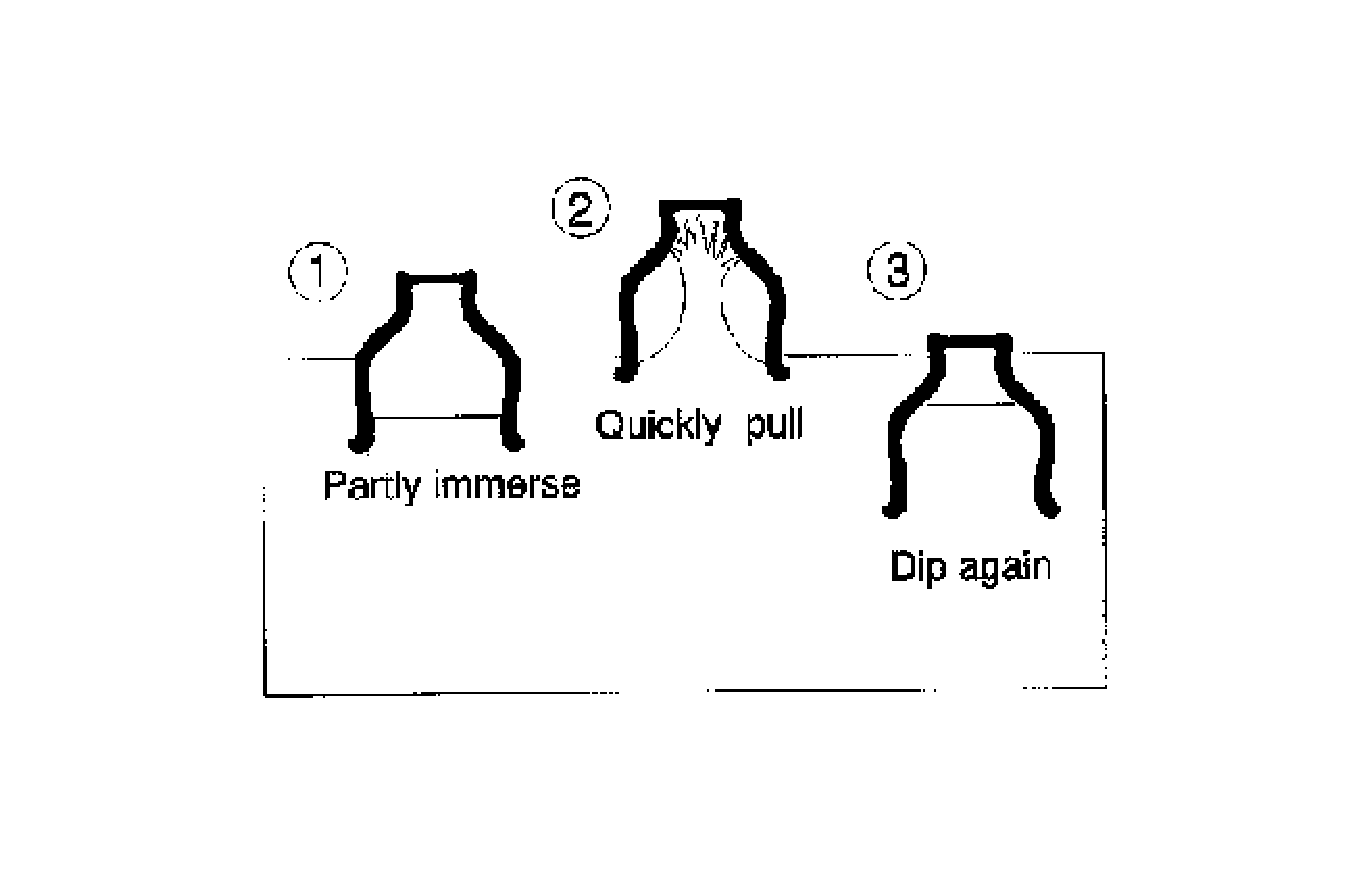
\includegraphics[width=0.7\linewidth]{img/glazingcup.eps}
  \caption{Three steps of glazing the inside and outside of a cup in one dip.}
  \label{fig:glazingcup}
\end{figure}
%-------------------------------------------------------------------------------
\subsubsection{Tiles}
To dip tiles, hold them by the edges and dip them in the glaze while moving 
sideways. This also requires practice!
%-------------------------------------------------------------------------------
\begin{figure}[htbp!]
  \centering
  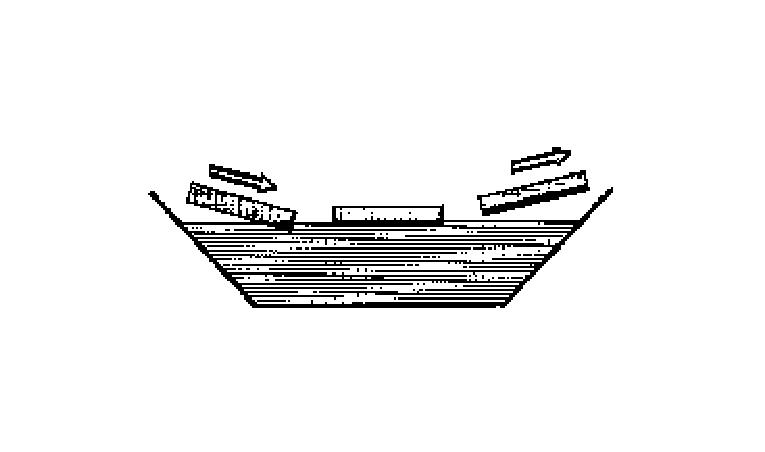
\includegraphics[width=0.7\linewidth]{img/glazingtile.eps}
  \caption{Dipping tiles in glaze.}
  \label{fig:glazingtile}
\end{figure}
%-------------------------------------------------------------------------------
\subsubsection{Double Dipping}
Applying a second coat of the same or a different glaze over the first is known 
as double dipping. This often happens inadvertently. When glazing the inside, 
sometimes there will be runs of glaze on the outside. These should be sponged 
clean before doing the outside. Larger items are often partly dipped to cover 
the top, then turned over and dipped again to coat the bottom. This usually 
results in a line of double glaze, which will look different. If the 
overlapping area is chosen carefully, it can become a part of the design. 
Otherwise, it will look like a mistake.

For decorative effects, a pot is sometimes dipped partly in one glaze and then 
again in a different glaze. This results in a third color where the two overlap.
%-------------------------------------------------------------------------------
\subsubsection{Waterfall Glazing}
In the commercial glazing of tiles, the ``waterfall'' system is used. This 
consists of a conveyor belt, which carries the tiles under a thin waterfall of 
glaze that pours over them. The thickness of application is controlled by the 
speed of the conveyor belt and the amount of glaze flow. Excess glaze runs into 
a tank, which is again pumped up to the waterfall. These machines are often 
equipped with automatic cleaners that take excess glaze off the sides of the 
tiles.
%-------------------------------------------------------------------------------
\begin{figure}[htbp!]
  \centering
  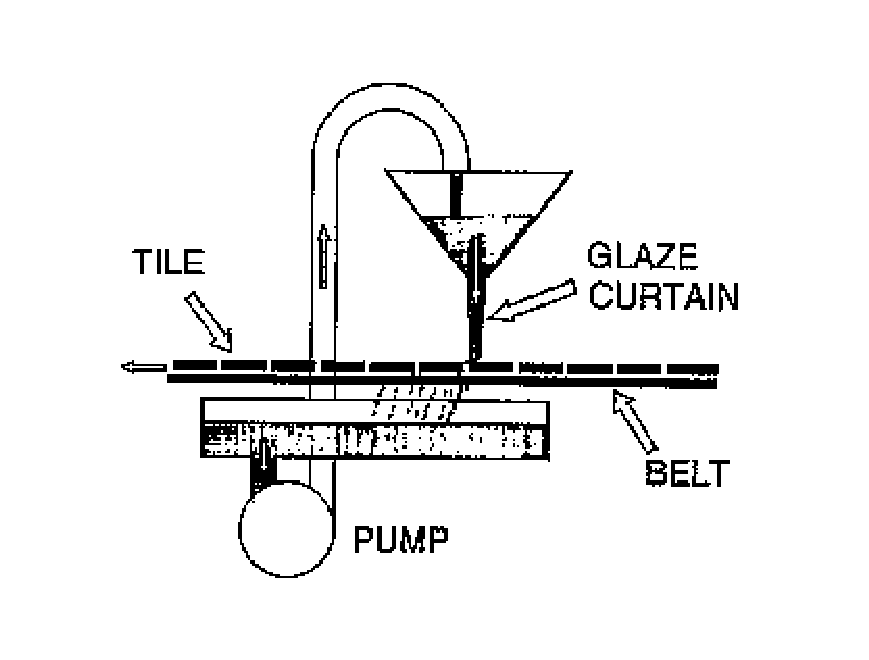
\includegraphics[width=0.7\linewidth]{img/glazingwaterfall.eps}
  \caption{Waterfall glazing of tiles. The tiles run through a curtain of glaze 
  which is continuously recycled with the help of a pump.}
  \label{fig:glazingwaterfall}
\end{figure}
%-------------------------------------------------------------------------------
\subsection{Spraying}
Spraying is used for items that cannot easily be dipped or poured. It requires 
an air compressor and a spray gun, as well as a spray booth equipped with an 
exhaust fan. This is not recommended for the small producer, unless it is 
required for frequent use or for special decorative effects. Ordinary spray 
guns for paint can be used, but they wear out quickly because glaze is 
abrasive. Special spray guns for glaze are equipped with silicon carbide spray 
heads.

Spraying has the disadvantage of wasting a lot of glaze that goes into the air. 
This is dangerous to inhale, and a spray booth should be provided with an 
exhaust fan to the outside, as well as having a filter to catch excess glaze. 
If a great deal of spraying is done, the excess glaze can be collected from the 
filter and the inside of the booth and reused.

As usual, the inside of the item is glazed first (usually by pouring), and the 
spraying is done in several even, systematic coats. Each one must be applied 
before the first one dries, or the glaze may lift off the pot. Each coat should 
be lightly applied, so that it looks a bit powdery.

It is difficult to judge the correct thickness of glaze and to get it even all 
over, especially in difficult areas like under handles. In time the glazer will 
learn to measure the thickness by feeling it with a fingernail.
%-------------------------------------------------------------------------------
\subsubsection{Airbrush}
An airbrush is a very small spray gun that can be adjusted from a pencil-thin 
spray to a wide pattern. These are not used for glaze application, but are 
often used for decorative effects-with underglazes and overglazes.
%-------------------------------------------------------------------------------
\subsubsection{Care of the Spray Gun}
Spray guns are very sensitive. They tend to get clogged, so make sure that your 
glaze is sieved before putting it in the gun. Clean the spray gun immediately 
after use by rinsing it out and spraying clean water through it until there is 
no sign of glaze. Glaze left in the spray gun will corrode it and make it 
unusable.
%-------------------------------------------------------------------------------
\subsubsection{Glaze Fountain}
For glazing the inside of large items a glaze fountain as shown in 
figure~\ref{fig:glazingcup} is helpful. The pot is placed over a nozzle from 
which an electric pump provides a powerful upward shower of glaze when 
activated with a switch on the floor.
%-------------------------------------------------------------------------------
\section{Density, Binders, Glaze Thickness}
As described above, it is important to have the correct a nouns of water in 
your glaze. The glaze should always be checked and corrected by test dipping 
some biscuit before starting and then relying on your experience to judge if 
the thickness is correct. Checking specific gravity with a hydrometer or by 
weighing is a good practice but should not be relied on.

It is best not to use binders unless you have no choice. CMC gum is the most 
satisfactory.
%-------------------------------------------------------------------------------
\subsubsection{Non-porous Biscuit}
As previously mentioned, differences in biscuit firing temperature cause 
differences in porosity and can cause problems in glaze application. Overfired 
biscuit is especially difficult to glaze, as it will not absorb water. In the 
making of whiteware, the biscuit temperature is usually higher than the glaze 
temperature. This results in a semivitrified body that has special glaze 
application problems. If it is necessary to reglaze pots that have firing 
defects, they also require special handling.

If you only have a few pieces, they can be heated until almost too hot to 
handle and then dipped, poured or sprayed (spraying is most satisfactory). The 
heat will make excess water evaporate.

If glazing vitrified ware is part of your standard production, then it is best 
to flocculate your glaze. This is the opposite of deflocculation (as used with 
casting slip) and results in a thick, pudding-like glaze with the normal water 
content.
%-------------------------------------------------------------------------------
\section{Waxing}
In order to keep glaze from being applied to the foot of your pots, it is often 
more efficient to wax the bottoms as compared to sponging them clean. The 
coating of wax prevents glaze from sticking. There are two common waxing 
methods:
%-------------------------------------------------------------------------------
\subsubsection{Hot Wax}
Paraffin wax is kept melted in a shallow metal pan over an electric heater or 
a smoldering charcoal fire (an open fire should not be used as the paraffin 
may start to burn). It should be hot, but not so hot that it starts to smoke. 
Before applying the glaze, the foot rings are dipped in the paraffin.
%-------------------------------------------------------------------------------
\subsubsection{Liquid Wax Resist}
It is much easier to use liquid wax resist, which is a wax emulsion in a 
water base. It can be thinned with water but after drying cannot be 
dissolved. This is commercially available in some countries specifically for 
glaze application. It is also possible to use liquid floor wax.

Liquid wax resist is also used for decoration.
%-------------------------------------------------------------------------------
\section{Single-Fire Glazing}
Single-fire glazing is sometimes called ``raw glazing'', but this term is 
confusing as ``raw glaze'' also is used for unfritted lead or borax glazes. 
Glaze is applied directly to bone-dry or leather-hard ware and fired once up to 
the glaze temperature. Not all glazes and bodies are suitable for single 
firing, and each combination needs to be tested.

Glazes that work on biscuit ware will often also work on bone-dry clay with a 
small addition of a plastic clay or bentonite. Glazes for leather-hard glazing 
will need more clay so the glaze layer will shrink along with the clay during 
drying. The leather-hard method is less practical, since each batch of 
leather-hard pots must be glazed immediately, causing problems in the work flow.

The advantage of single firing is that it avoids the fuel and extra handling 
needed for biscuit firing. The main problem with single firing is crawling 
caused by different shrinkage rates of clay and glaze in the early stages of 
the firing. Single-fire glazes usually have a high percentage of clay.

Delicate ware cannot usually be single-fired successfully, as it tends to be 
damaged by the water.

Single-fire glazing needs to be done quickly and carefully, without letting 
glaze stand inside the pot for a long time. Dipping and pouring can be used, 
and spraying is also effective.

Firing needs to be done more slowly than usual, so that pots do not explode. 
The early stages of firing should be done as with biscuit firing.

Single firing is used most often in large tile industries, where it saves fuel.
%-------------------------------------------------------------------------------
\section{Handling, Drying Before Firing}
Good glaze application requires careful handling. Many pots are spoiled by 
fingerprints or glaze that is knocked off during handling. Pots should be 
allowed to dry before loading in the kiln.

The kiln loader should be responsible for checking each pot as he places it in 
the kiln. This means inspecting the foot to see if it is clean and rejecting 
pots with damaged or thick glaze. The loader should constantly clean his hands 
of glaze dust especially when loading ware with different colored glazes. 
Otherwise colored fingerprints will mark the pots.
%-------------------------------------------------------------------------------
\section{Salt Glazing}
In salt glazing, no glaze is actually applied to the pot before firing. The 
ware is single-fired up to the maturing point of the clay and rock salt is then 
introduced directly into the firebox. The salt breaks down into sodium and 
chlorine gas. The sodium combines with silica on the surface of the pot to make 
a durable glaze and the chlorine goes up the chimney, combining with water in 
the air to form hydrochloric acid. This is an irritant, as well as causing 
damage to vegetation and metal structures in the immediate vicinity. Another 
problem is that the salt erodes the firebricks in the kiln rather fast.

Salt glazing normally is done on stoneware at temperatures above 1100\degree C. 
Salt is often mixed with borax to lower the melting point (see also 
section~\ref{sec:meltingpointsec}).
%-------------------------------------------------------------------------------